\relatorio
{Engenharia de dados para plataforma de consultoria educacional}
{
    \noindent Pesquisadores: Gabriel Araújo Alves, Gustavo Cavaletti e Felipe Bakowski Nantes de Souza
    
    \noindent Orientador: José Renato Garcia Braga
}
{
    Este trabalho aborda a Engenharia de Dados no contexto do processo de qualidade de dados. Além disso, representa uma colaboração com a empresa FRST Falconi, que proporcionou suporte integral em termos de orientação e disponibilização de material (dataset). O objetivo dessa parceria é explorar soluções que aprimorem a eficiência do processo de qualidade de dados na empresa, proporcionando aos tomadores de decisão um ambiente de trabalho facilitado e dados de alta qualidade.
}
{Engenharia de dados, Qualidade de dados, Big Data}

\section{Introdução}

Na era digital, onde os dados se tornaram ativos essenciais para o sucesso corporativo, a Engenharia de Dados desponta como uma disciplina-chave para moldar o futuro das organizações. Este trabalho se dedica à aplicação da Engenharia de Dados para aprimorar o processo de qualidade de dados, em parceria com a empresa FRST Falconi.

O objetivo é compreender e catalisar melhorias que fortaleçam a eficiência do processo de qualidade de dados, proporcionando à FRST Falconi uma base sólida de dados para tomada de decisões.

Além disso, é notório inferir que o trabalho apresentado será de grande valia e servirá como alicerce para o processo de ciência de dados realizado por outro projeto, também em parceria com a FRST Falconi.

\section{Motivação}

A formalização do ambiente digital pelo mercado corporativo dá luz ao problema de organização de informaçoes úteis para as empresas, em que o custo de acesso à dados de qualidade pode ser reduzido ao fazer uso de ferramentas de engenharia de dados. O desperdício de tempo dos cientistas de dados, por ano, com desafios de limpeza e organizaçao de dados é de cerca  de 60\%. Além disso, anualmente US\$ 3.1 Trilhões são desperdiçados anualmente com tarefas oportunas à prática de engenharia de dados por causa de dados recebidos com baixa qualidade.


\section{Problema}

Compreender o funcionamento e falhas do processo de ingestão de dados da FRST é o objetivo principal desse trabalho, em vista de possibilitar a decodificação do caminho dos dados para elencar onde e quando as falhas ocorrem e assim possibilitar a correção. O resultado final será um dashboard de visualização das falhas com uso de gráficos de tempo e contagem de erros para demonstrar quando a falha ocorreu. A forma como a falha é representada também pode servir de indicativo para a parte do processo que resultou no erro. A exemplo, um dos gráficos demonstrou triplicação dos dados enviados à camada raw, assim, encontramos uma falha que após cópia dos dados da base de produção, fora enviado três vezes a mesma cópia. 

\section{Qualidade de dados}

Qualidade de dados é o processo pelo qual se desenvolvem ferramentas de avaliação e tratamento das informações de uma base de dados para adequá-la à métricas de qualidade.
A avaliação engloba análise da precisão dos dados, ou seja, quanto esse dado representa a realidade, a exemplo avalia-se a base de uso do cientista de dados se possui informações corretas em relação à quantidade de desafios completada pelos usuários. Com informações precisas, exige-se também a consistência desse trânsito correto de informações entre as diferentes fontes de dados, por exemplo analisa-se essa informação de quantidade de desafios completada se é exibida de maneira igual entre as diferentes fontes de uso desses dados. Integridade e confiabilidade também são aspectos relevantes para a engenharia de dados, visto que uma base de dados precisa estar completa, sem dados faltantes e ter origem de fontes confiáveis, na FRST, as informações são coletadas da própria base de produção, essa que poucas pessoas possuem acesso cujo propósito é propor confiabilidade aos dados da empresa. Além disso, a a métrica de atualidade é relevante ao proporcionar as informações em tempo hábil para empresa, por exemplo, leva-se cerca de um dia para viabilizar a quantidade de dados necessária para tomadas de decisão na FRST, enquanto em corridas de Fórmula 1 a informação deve ser repassada do piloto à equipe em milésimos de segundo e em bancos a informação pode levar até mesmo semanas para se tornar hábil ao uso.

\section{Processo de qualidade de dados}

De início, todo comportamento de um usário é registrado em uma base de dados de produção, ademais,  o comportamento que nos interessa é a conclusão ou começo de desafios, quando um desafio é iniciado ele é adicionado na base e quando ele é deletado, atribui-se uma característica de 'deletado', mas, sem efetivamente o deletar. Em seguida, essa base é copiada, utilizando Amazon glue, e armazenada na camada raw da Amazon S3. Então, ocorre o processo de qualidade de dados na cópia e armazenamento dos dados da camada raw para a trusted. 

Nessa medida, esse processo consiste em garantir que os dados de ambas as camadas estejam congruentes, ao verificar se não houve alguma repetição desnecessário ou corrompimento. Tal procedimento é feito em Python e pode ser reduzido à contagem de elementos em ambas os dados e na validação dessa contagem (verificar se estão iguais)

Por fim, pode-se visualizar esse processo completo na imagem abaixo:
    \begin{figure}[h!]
        \centering
        \caption{Qualidade dados}
        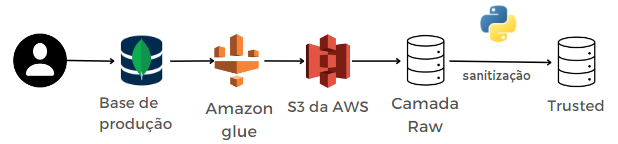
\includegraphics[width = .6\linewidth]{relatorios/grupo5/figuras/qualidade_dados.png}
        \label{Processo}
    \end{figure}

\section{Hipótese e Objetivos}

Tendo como a base a intuição construída, é possível formular a hipótese de que o erro ocorre durante o processo de cópia da base de produção para a raw ou no processo de qualidade dos dados. Assim, para validarmos essa hipótese iremos construir gráficos, utilizando superset, que comparam as informações da base de produção e na camada trusted. Dessa maneira, é possível validar a existência desse erro empíricamente.

\section{Resultados}

Na figura 2, pode-se observar, na base de produção, a contagem de desafios deletados, atuais e o total (atuais + deletados).
    \begin{figure}[h!]
        \centering
        \caption{Total Desafios}
        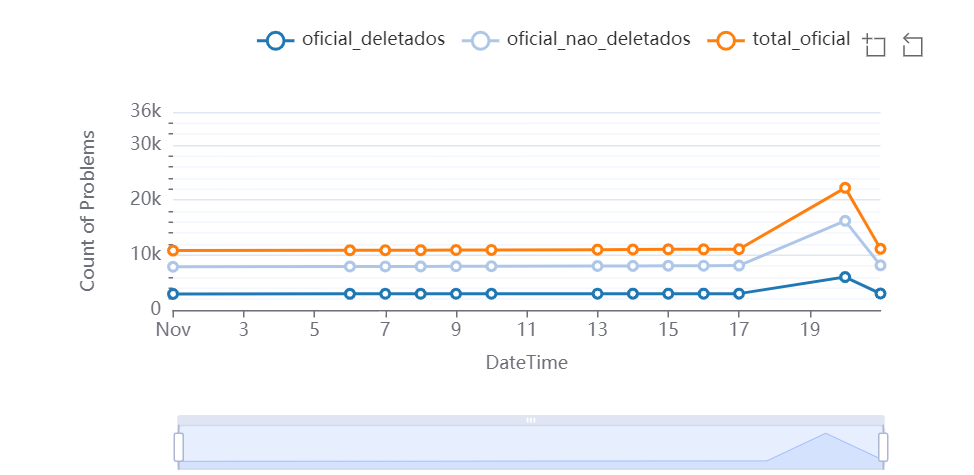
\includegraphics[width = 1\linewidth]{relatorios/grupo5/figuras/result1.png}
        \label{Cont Total}
    \end{figure}
        
Na figura 3, pode-se observar a diferença de desafios deletados, atuais e totais entre a base de produção e a camada trusted.
    \begin{figure}[h!]
        \centering
        \caption{Diferença Desafios}
        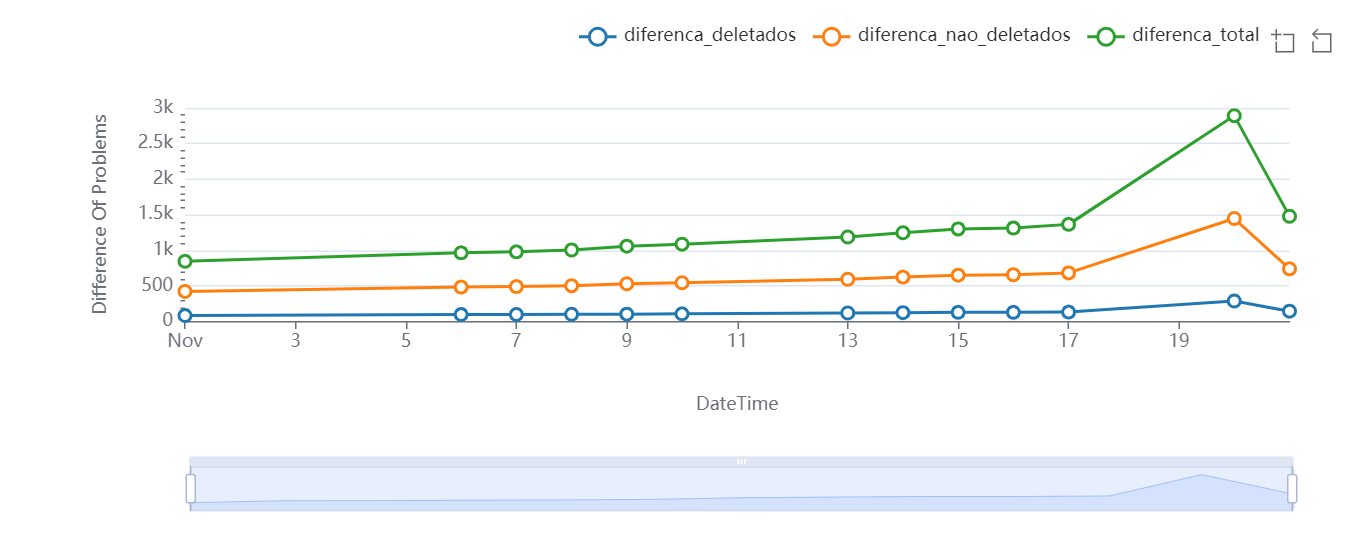
\includegraphics[width = 1\linewidth]{relatorios/grupo5/figuras/result2.png}
        \label{fig:mapa}
    \end{figure}

Analisando essas 2 figuras, foi possível perceber uma anomalia, na qual, a base teve um erro de cópia que resultou nela tendo suas informações duplicadas. Fato que foi possível observar graças a esses gráficos. Ademais, pode-se perceber que a diferença entre as duas bases continua a crescer.

A seguir, podemos visualizar uma tabela (figura 4) que mostra cada um dos criterios da figura 3, mas, para o dia atual.

    \begin{figure}[h!]
        \centering
        \caption{Diferença Desafios - Dia Atual}
        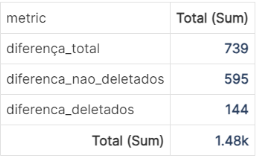
\includegraphics[width = 0.4\linewidth]{relatorios/grupo5/figuras/result3.png}
        \label{fig:mapa}
    \end{figure}

Por fim, a figura 5 é uma sequência de imagens, em que, a mais à esquerda representa a porcentagem de empresas com uma incongruência na base, a central é a porcentagem de empresas sem uma incongruência e a última é um histograma da contagem de erros em cada empresa.

    \begin{figure}[h!]
        \centering
        \caption{Análise de erros}
        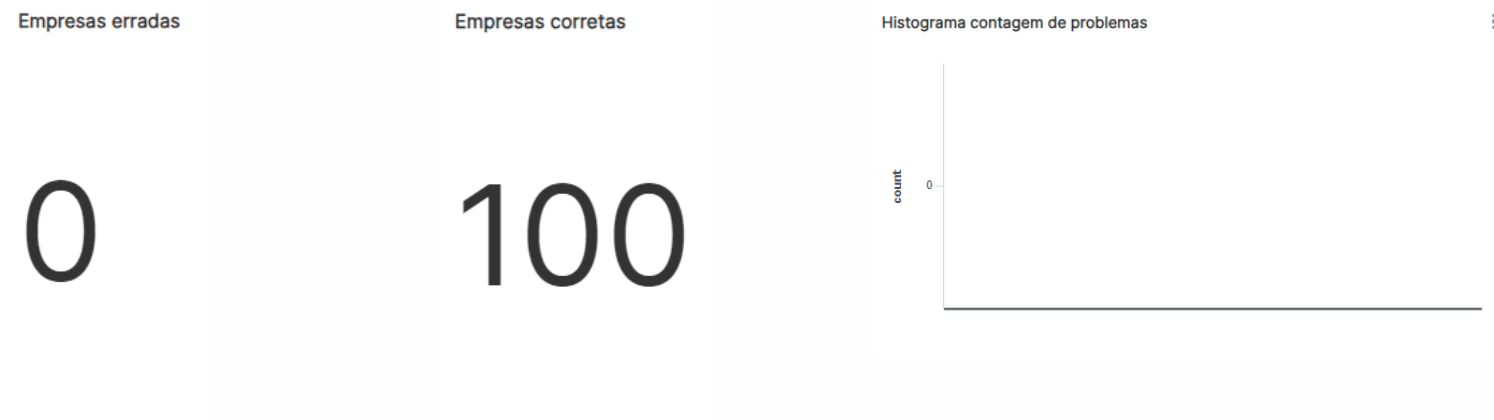
\includegraphics[width = 0.8\linewidth]{relatorios/grupo5/figuras/results4.png}
        \label{fig:mapa}
    \end{figure}    

Assim, fica mais eficiente achar em que parte da base ocorreu um erro, pois, aponta diretamente para a empresa. Nessa medida, salva-se muito tempo diagnosticando o erro.

\section{Conclusão}

Em resumo, a integração de Engenharia de Dados e Qualidade de Dados apresenta-se como um diferencial estratégico para a FRST Falconi. Este trabalho não só destaca as capacidades transformadoras dessas disciplinas, mas também sinaliza um futuro no qual dados de qualidade impulsionarão decisões corporativas mais informadas. 

Ao consolidar essa abordagem, firma-se um compromisso de contribuir para fortalecer o ecossistema de ciência de dados na parceria contínua com a FRST Falconi. 

Neste sentido, há um cenário onde os dados não apenas informam, mas capacitam a tomada de decisões empresariais mais precisas e estratégicas.

Logo, é de fundamental importância entender o sentido do processo de tornar os dados confiáveis, eficientes, precisos, integros e atuais para a melhor tomada de decisão.
\section{Referências}
    \begin{itemize}
        \item V. Mayer-Schonberger and K. Cukier, Big Data: A revolution that will transform how we live, work, and think. Houghton Mifflin Harcourt, 2013.
        \item J. R. GalbRaith, Organizational Design Challenges Resulting From Big Data, Journal of Organisation Design, Apr 2014
        \item https://hbr.org/2016/09/bad-data-costs-the-u-s-3-trillion-per-year
        
    
    \end{itemize}
\section{Ferramentas}
    \begin{itemize}
        \item 
        Amazon Web Services: S3 e Athena são os serviços da AWS utilizados neste projeto e que servem para armazenar os dados que foram trabalhados.
       
        \item MongoDB: Banco de dados NoSQL também responsável por armazenar os dados, no entanto, neste caso, o MongoDB é a base original de produção da empresa onde estão todos os desafios propostos por clientes.
        
        \item Python : linguagem em que houve o desenvolvimento da aplicação.
        
        \item Airflow: ferramenta responsável por construir pipelines de dados que são etapas afim de avaliar quaisquer erros do código desenvolvido.
    
        \item Superset: responsável pela construição do produto final, ou seja, o dashboard de visualização de dados.
    
    \end{itemize} 

